\section{Base di dati sistema logging}\label{sec:sbd-sistema-logging}

\subsection{Abstract}

L’obiettivo è sviluppare un servizio che tenga traccia in maniera intelligente dei log. Questo servizio offre numerosi benefici legati alla retrospettiva. Il miglioramento delle prestazioni del sistema, la risoluzione rapida dei problemi, il rilevamento delle minacce alla sicurezza e la generazione di informazioni utili per l'analisi e il miglioramento continuo sono solo alcuni dei benefici che questo servizio permette.

\subsection{Analisi dei requisiti}

\subsection{Progettazione concettuale}

\subsubsection{Analisi delle entità}

\textbf{Se non specificato l'attributo è NOT NULL}

%LOG
\begin{center}
    \begin{tabularx}{\textwidth}{|l|l|l|X|}
        \hline
        \rowcolor{gray!30}
        \multicolumn{4}{|c|}{\textbf{LOG}}\\
        \hline
        idMisuratore & INTEGER & Identifica univocamente, insieme a {\it{time}}, un log & Chiave\\
        \hline
        istanteModifica & LONG & Indica quando c'è stata una variazione ad un lampione o ad un sensore & Chiave\\
        \hline
        valore & INTEGER & \multicolumn{2}{l|}{Nel caso di un sensore, indica se è in grado di rilevare persone oppure no} \\
        & & \multicolumn{2}{l|}{Nel caso di un lampione, indica il suo valore di luminosità} \\
        \hline
        tipo & VARCHAR(50) & \multicolumn{2}{l|}{Indica se il sistema sta facendo riferimento ad un sensore oppure ad un lampione} \\
        \hline
    \end{tabularx}
\end{center}

\subsubsection{Schema ER concettuale}

\begin{center}
    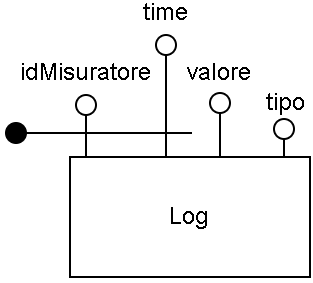
\includegraphics[width=4.5cm]{contenuti/specifica-basi-dati/img-sbd/logging_concettuale.png}
\end{center}

\subsection{Progettazione logica}

\subsubsection{Schema concettuale ristrutturato - Schema Logico}

\begin{center}
    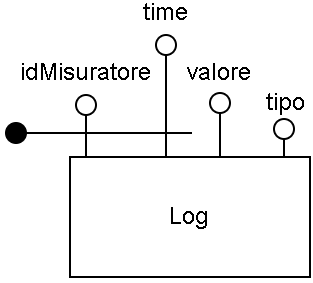
\includegraphics[width=4.5cm]{contenuti/specifica-basi-dati/img-sbd/logging_logico.png}
\end{center}

\subsubsection{Descrizione schema relazionale}

Per questione di compatibilità con il DBMS alcuni nomi di attributi entità e relazioni sono stati normalizzati, utilizzando il camelCase, togliendo gli accenti, accorciando i nomi molto lunghi e con altre piccole accortezze.
La chiave primaria è indicata in \textbf{grassetto}, le chiavi esterne sono indicate con la \underline{sottolineatura}.

\textit{Log}(\textbf{idMisuratore}, \textbf{time}, valore, tipo)
